\subsection{Реляционная алгебра. Деление и операции над данными}

\subsubsection{Деление}

\begin{definition}
	\textit{Делением}	называется операция, результат которой $R(X) = Q(XY) \div S(Y)$
	максимальный при условии $R \times S \subseteq Q$. Эту операцию можно записать по-другому:
	\begin{itemize}
		\item $Q \div S \equiv \{\,x \mid x \in \pi_X(Q),~ \{x\} \times S \subseteq Q\,\}$.
		\item $Q \div S \equiv \pi_X(Q) \setminus \pi_X(\pi_X(Q) \times S \setminus Q)$.
	\end{itemize}
	Заголовок результирующего отношения -- X. $S \subseteq Q$.
\end{definition}

\begin{remark}
	Интуитивно, эта операция -- запрос всех $X$ таких, что для всех
	$Y$ найдется пара, равная по $X$: $x \in \pi_X(Q)\colon~ \forall y \in S\colon~ (x, y) \in Q$.
\end{remark}

На рисунке \ref{div-ex} представлен пример деления.

\begin{figure}[H]
	\centering
	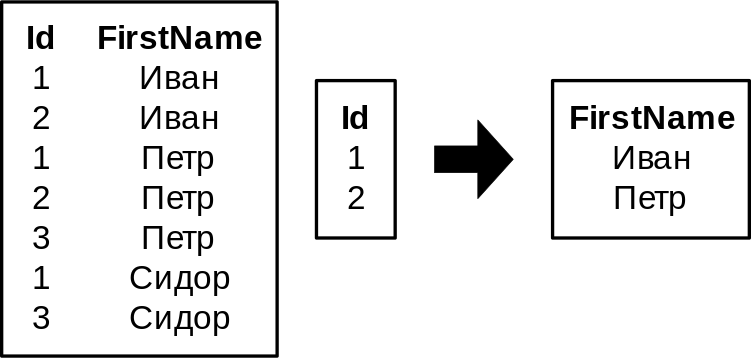
\includegraphics[width=0.8\textwidth]{../assets/kgeorgiy/relalgebra/Divide_Example_2.svg.png}
	\caption{Пример деления}
	\label{div-ex}
\end{figure}

\subsubsection{Большое деление}

\begin{definition}
	\textit{Большим делением} называется операция, которую можно представить следующим образом:
	\begin{itemize}
		\item $Q(XY) \gdiv S(YZ) \equiv \{\,(x, z) \mid \{x\} \times \pi_Y(\sigma_{Z=z}(S)) \subseteq Q \,\}$.
		\item $Q(XY) \gdiv S(YZ) \equiv \pi_X(Q) \times \pi_Z(S) \setminus
			      \pi_{XZ}(\pi_X(Q) \times S \setminus Q \bowtie S)$.
	\end{itemize}
	Заголовок результирующего отношения -- XZ.
\end{definition}

\begin{remark}
	Интуитивно, большое деление -- запрос `для всех связанных', или деление для каждого
	$z$. Иначе говоря, для каждого $z$ найти такие
	$x$, что для всех $y$, связанных с $z$,
	найдется соответсвующий $x$: \[
		(x, z) \in \pi_X(Q) \times \pi_Z(S)\colon~ \forall y \in
		\pi_Y(\sigma_{Z=z}(S))~~ (x, y) \in Q.
	\]
\end{remark}

На рисунке \ref{gdiv-ex} представлен пример большого деления.

\begin{figure}[H]
	\centering
	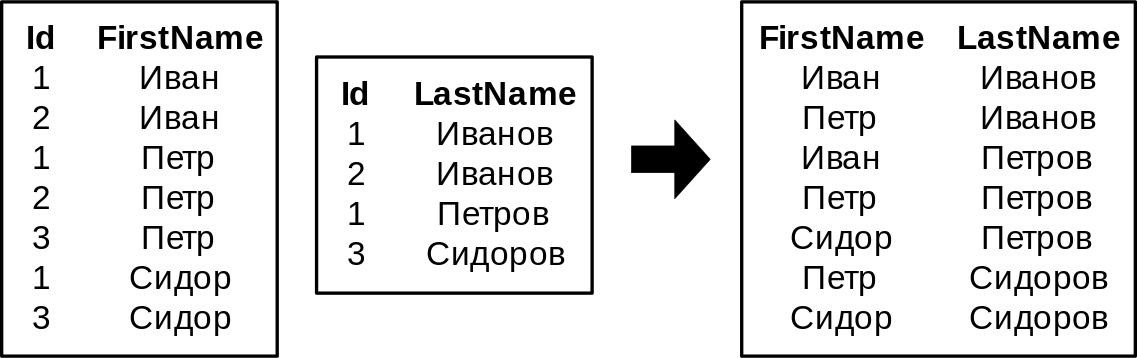
\includegraphics[width=0.8\textwidth]{../assets/kgeorgiy/relalgebra/Divide_Great_Example_2.svg.png}
	\caption{Пример большого деления}
	\label{gdiv-ex}
\end{figure}

\subsubsection{Расширение}

\begin{definition}
	\textit{Расширение} -- операция над данными, добавляющая новый вычисляемый атрибут. Заголовком
	результата будет $R \cup \{A\}$. Обозначение: $\e_{A=\texttt{expr}}(R)$. К каждому кортежу
	тела $R$ добавится вычисленное значение \texttt{expr}. Выражением может
	быть комбинация атрибутов $R$, а также различные функции и операции, доступные в
	БД.
\end{definition}

На рисунке \ref{extend-ex} изображен пример композиции расширений $\e_{\texttt{Tax}=\texttt{tax10(Total)}}
	\circ \e_{\texttt{Total}=\texttt{Price} \cdot \texttt{Items}}$.

\begin{figure}[H]
	\centering
	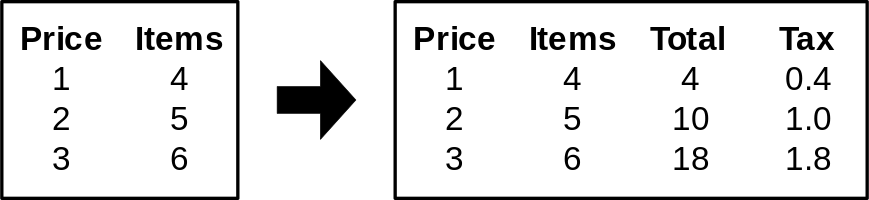
\includegraphics[width=0.8\textwidth]{../assets/kgeorgiy/relalgebra/Data_Extend_2.svg.png}
	\caption{Пример расширения}
	\label{extend-ex}
\end{figure}

\subsubsection{Агрегирование}

\begin{definition}
	\textit{Агрегирование} -- обработка набора значений. Обозначается $\texttt{func}_{Q,A}(R)$.
	\begin{itemize}
		\item Примеры \texttt{func}: \texttt{count, sum, avg, max, min, all, any}.
		\item Q -- агрегируемый атрибут.
		\item A -- сохраняемые атрибуты.
		\item $r \in \pi_A(R)$ расширяется атрибутом $Q = \texttt{func}(\pi_Q\{\,q \in R \mid \pi_A(q) = r\,\})$
	\end{itemize}
\end{definition}

\begin{remark}
	Интуитивно, данные разбиваются по корзинам с одинаковыми $A$, после чего
	каким-то образом сворачиваются,  то есть, на каждой корзине по отдельности считается заданная
	функция.
\end{remark}

На рисунках \ref{aggr-ex-1}, \ref{aggr-ex-2} изображены примеры агрегирования.

\begin{itemize}
	\item $\texttt{sum}_{\texttt{Total},\{\texttt{Supplier}\}} \circ
		      \e_{\texttt{Total}=\texttt{Price} \cdot \texttt{Items}}$
	      \begin{figure}[H]
		      \centering
		      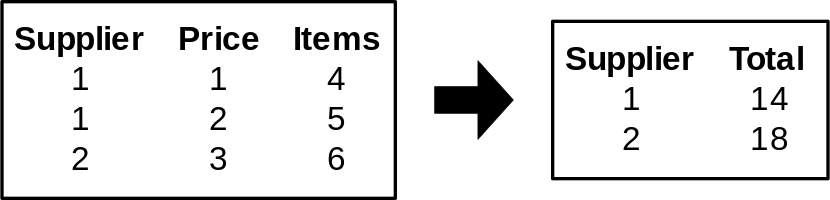
\includegraphics[width=0.8\textwidth]{../assets/kgeorgiy/relalgebra/Data_Aggregate_1_2.svg.png}
		      \caption{Пример агрегирования 1}
		      \label{aggr-ex-1}
	      \end{figure}
	\item $\texttt{sum}_{\texttt{Total},\varnothing} \circ \e_{\texttt{Total}=\texttt{Price} \cdot \texttt{Items}}$
	      \begin{figure}[H]
		      \centering
		      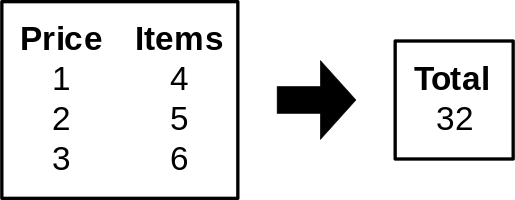
\includegraphics[width=0.8\textwidth]{../assets/kgeorgiy/relalgebra/Data_Aggregate_2_2.svg.png}
		      \caption{Пример агрегирования 2}
		      \label{aggr-ex-2}
	      \end{figure}
\end{itemize}

